\chapter{Análise Bibliográfica sobre o Uso de Big Data na Política, por Enzo Nunes Leal Sampaio}

\section{Planejamento do estudo}
Política, do grego \textit{politikos} significa algo relacionado com grupos sociais que integram a Pólis \citep{wikipedia_politica_nodate}. Diante dessa definição podemos assumir que a política faz parte do dia a dia de todas as pessoas.

A partir desse pensamento foi questionado sobre a participação da computação nesse tema. Mais especificamente, como o Big Data pode influenciar na política.

Dessa forma, os questionamentos que norteiam este estudo são:

\begin{itemize}
    \item Qual a base de conhecimento produzida sobre o tema de Uso de Big Data na Política?
    \item Como os partidos políticos usam o Big Data em suas campanhas?
    \item Como certos grupos políticos podem se beneficiam do uso de Big Data?
\end{itemize}

\subsection{Uso do Bibliometrix e Biblioshiny}

O Bibliometrix é uma biblioteca da linguagem R que permite a realização de análises quantitativas e estatística sobre publicações científicas.

O Biblioshiny é uma ferramenta do pacote Bibliometrix que contribui com aspectos visuais às funções executadas pela biblioteca.

A pesquisa bibliográfica sobre o tema já mencionado é feita usando, principalmente, essas duas ferramentas.

\subsection{Limitações}
O estudo foi feito em uma semana com trabalhos de duração de uma hora por dia e utilizando somente a base de dados Web of Science(WoS).

\section{Coleta de dados\label{BDP:coleta}}
A coleta de dados foi feita a partir da base Web of Science no dia 3 de fevereiro de 2022, acessado pelo Portal de Periódicos da CAPES. As buscas foram feitas nas coleções Science Citation Index Expanded(SCI-EXPANDED) e Social Sciences Citation Index (SSCI) com foco nas categorias relacionadas às ciências exatas e foram obtidos 2093 registros. A pesquisa pode ser vista a seguir:

\lstinputlisting[numbers=left,basicstyle=\normalsize\ttfamily]{experiments/enzodevs2000/AnaliseBibliometrica/BigDataInPolicy/busca.tex}

\subsection{Explicações para os termos de busca usados\label{BDP:query}}
Como o objetivo é buscar registros que relacionem \textbf{Big Data} e \textbf{Política} é feita uma conjunção entre duas cláusulas principais, sendo que, na primeira tem-se uma outra cláusula conjuntiva entre as palavras \textit{big} e \textit{data}. Já na segunda cláusula principal tem-se uma disjunção entre 4 cláusulas.

A primeira é uma disjunção entre \textit{politica} e \textit{parties}. A segunda é \textit{elections}. A terceira é uma disjunção entre \textit{party} e \textit{campaigns}. Essas três cláusulas são feitas tendo como objetivo obter registros que ajudem a responder o segundo questionamento feito na primeira seção deste texto.

Por fim, a última cláusula \textit{policy} busca associar todos os temas já relatados com política.

\section{Análise dos dados}

\subsection{Filtragem de registros}
Antes de prosseguir com a análise, uma filtragem dos registros é feita para que se tenha como resultado somente registros de artigos publicados em revistas científicas. Dessa forma, com os 2097 registros inicias, chega-se, no final, ao número de 1834 registros.

\subsection{Análise descritiva do \textit{dataset}  BDP@enzodevs2000}

Com o auxilio do pacote Bibliometrix e de sua ferramenta visual Biblioshiny. Pode-se chegar as seguintes informações sobre o \textit{dataset}:

\begin{description}
    \item [\textit{Timespan}] Entre os registros obtidos após a filtragem tem-se artigos publicados no período de 1992 a 2022
    \item [\textit{Sources (Journals, Books, etc)}] Obteve-se 510 fonte diferentes para a origem dos registros
    \item [\textit{Average years from publication}] A média do tempo de publicação dos artigos é de 3.97 anos.
    \item [\textit{Average citations per documents}] Cada artigo do \textit{dataset} foi citado em média 17.31 vezes.
    \item [\textit{Average citations per year per doc}] Após a publicação do 1834 artigos, eles foram citados, em média, 2971 vezes.
    \item [\textit{References}] O total de artigos obtidos possuem juntos 80339 referências citadas.
    \item [\textit{Keywords Plus (ID)}] foram obtidos 3579 palavras-chave do tipo Keywords Plus (ID).
    \item [\textit{Author's Keywords (DE)}] 5754 palavras-chave indicadas pelos autores foram encontradas nos registros  .
    \item [\textit{Authors}] 11877 nomes de autores foram encontrados no \textit{dataset}  
    \item [\textit{Author Appearances}] Os 11877 distintos autores foram encontrados 14140 vezes, como autores de artigos.
    \item [\textit{Authors of single-authored documents}] Dentre os 11877 autores encontrados, 174 deles editaram artigos individualmente.
    \item [\textit{Authors of multi-authored documents}] Dentre os 11877 autores encontrados, 11703 deles editaram artigos com um ou mais co-autores.
    \item [\textit{Single-authored documents}] Dentre os 1834 artigos encontrados  \textit{dataset}, 175 foram escritos por um único autor.
    \item [\textit{Documents per Author}] Entre os 11877 autores, cada um publicou em média 0.154 documentos.
    \item [\textit{Authors per Document}] Cada um dos 1834 artigos encontrados no \textit{dataset} foi autorado, em média, com 6.48 autores.
    \item [\textit{Co-Authors per Documents}] As 14140 aparições autores se distribuem, em média 7.71 vezes para os 1834 documentos.
    \item [\textit{Collaboration Index}] Os 11703(nomes de) autores que editaram artigos com um ou mais co-autores, colaboraram em media 7.05 vezes.
\end{description}

\subsection{Evolução da produção científica}

Usando o Bibliometrix pode-se obter um gráfico que mostra a produção científica anual sobre o tema em questão. O gráfico obtido é o seguinte:

\begin{figure}
    \centering
    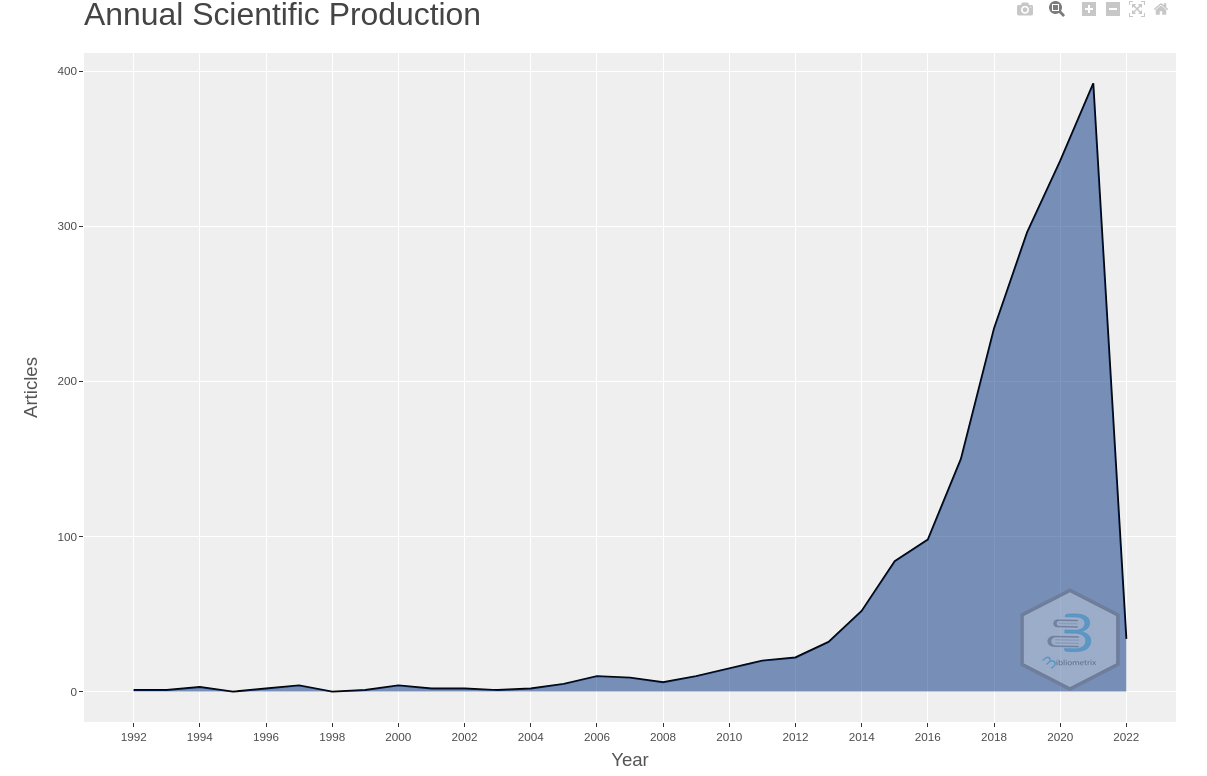
\includegraphics[width=1\textwidth]{experiments/enzodevs2000/AnaliseBibliometrica/BigDataInPolicy/Graficos/evolution.png}
    \caption{Evolução da produção científica no \dataset\   BDP@enzodevs2000}
    \label{fig:enzodevs2000:BDP:evol}
\end{figure}

Como pode-se ver na figura \ref{fig:enzodevs2000:BDP:evol}, o crescimento da produção científica sobre o tema de "Usos de Big Data na Política" vem crescendo exponencialmente de forma que a sua taxa de crescimento anual está em 13.42\%.

\subsection{Interpretação do crescimento \label{enzodevs2000:interpret_cresc}}

Pode-se interpretar que o crescimento exponencial da produção científica nesse tema represente um grande interesse por parte da comunidade acadêmica. Tal fato é compreensível, visto que, nos últimos anos tem-se tornado público alguns escândalos envolvendo o uso de dados obtidos para influenciar eleições políticas como pode ser visto neste artigo \citet{wikipedia_escandalo_nodate}.

\subsection{Evolução das citações}

\begin{figure}
    \centering
    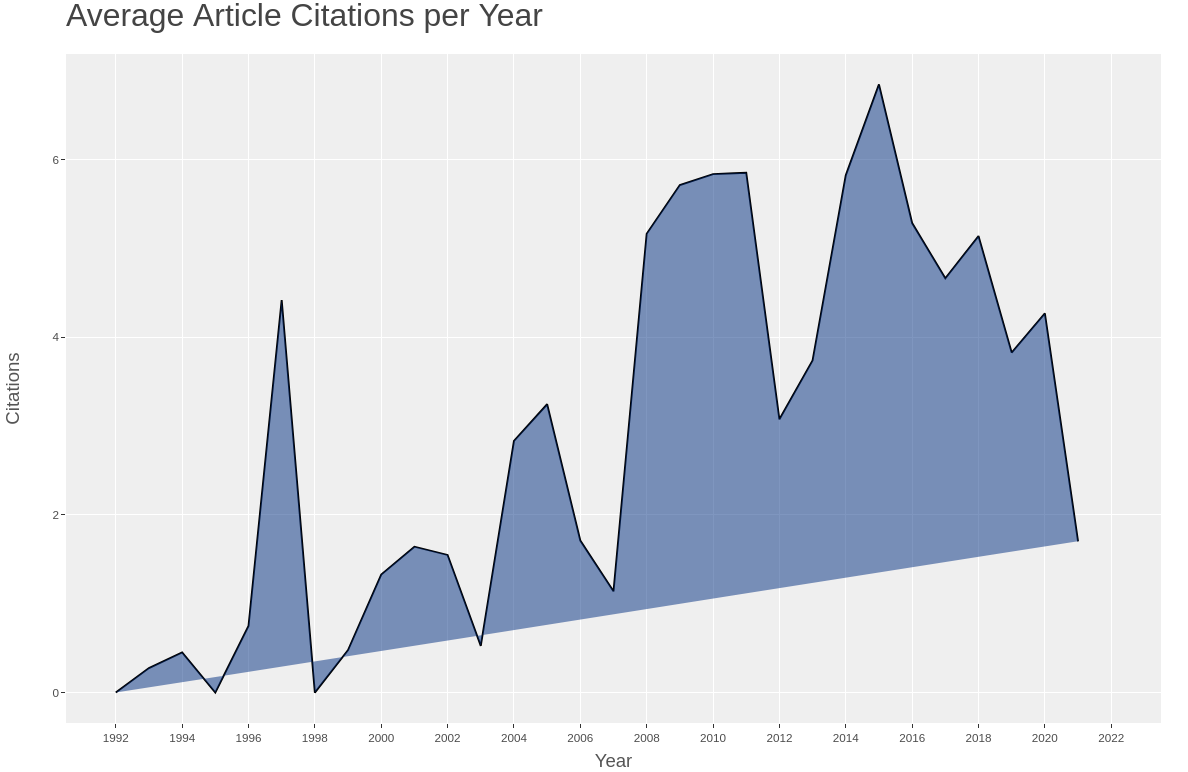
\includegraphics[width=1\textwidth]{experiments/enzodevs2000/AnaliseBibliometrica/BigDataInPolicy/Graficos/citations-evolution.png}
    \caption{Evolução das citações no \dataset BDP@enzodevs2000}
    \label{fig:enzodevs2000:BDP:evol_citation}
\end{figure}

Verifica-se, na figura \ref{fig:enzodevs2000:BDP:evol_citation} subidas e descidas quanto ao número de citações por ano, sendo o pico, o ano de 2015 quando se obteve o valor de 6.8 citações por ano.

\subsection{Interpretação da evolução das citações}

Como já mencionado, o pico de citações foi no ano de 2015. Ano em que as suspeitas sobre o uso de dados para influenciar eleições políticas começaram. Outro ano que teve uma expressiva quantidade de citações foi 2018 com um valor de 5.1 citações por ano. 2018 foi, também, o ano que grandes jornais fizeram reportagens mais detalhadas sobre o Escândalo de dados Facebook–Cambridge Analytica \citep{wikipedia_escandalo_nodate}.

\subsection{\textit{Three-Field Plots (Sankey diagram)}}

A seguir foi obtido um gráfico de 3 campos \ref{fig:enzodevs2000:BDP:3plotRAK}, no qual, pode-se visualizar 20 opções de cada. Sendo à esquerda as maiores citações, no meio os autores que mais contribuíram à direita as palavras-chaves mais utilizadas no registro.

\begin{figure}[h]
    \centering
    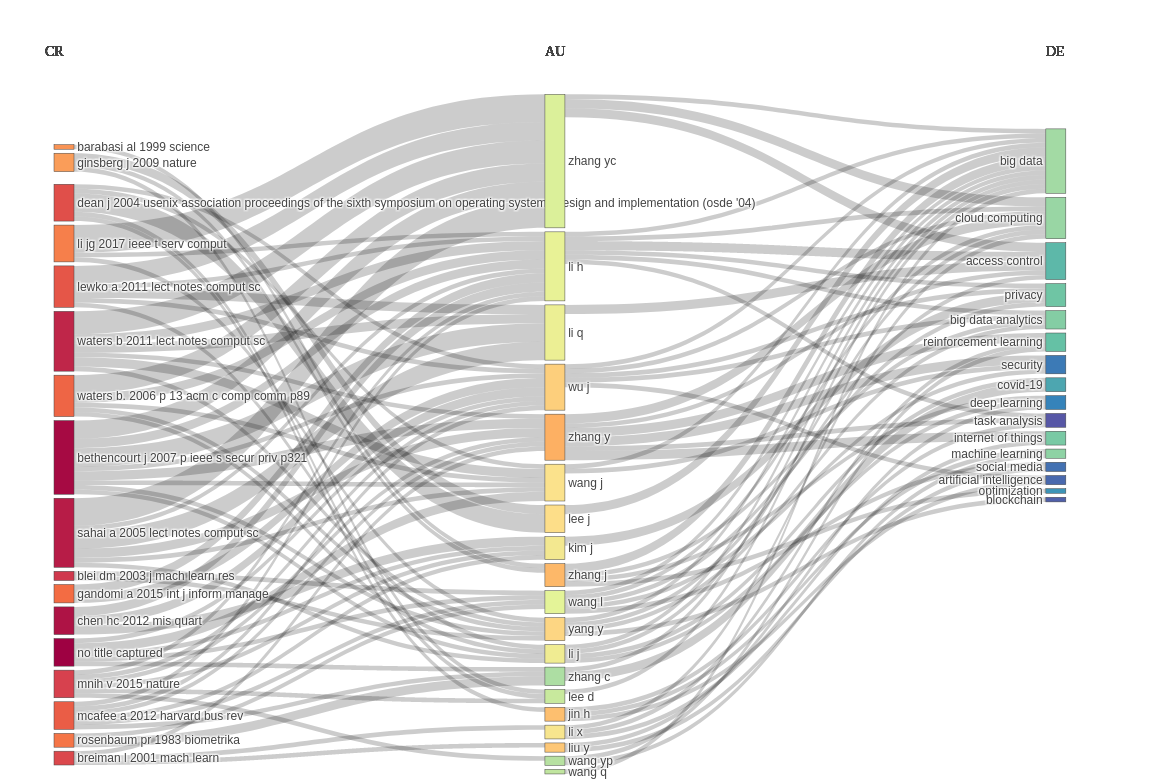
\includegraphics[width=1\textwidth]{experiments/enzodevs2000/AnaliseBibliometrica/BigDataInPolicy/Graficos/references_authors_keywords.png}
    \caption{Gráfico de 3 campos envolvendo os parâmetro Citações, Autores, Palavras-Chave do \dataset\ BDP@enzodevs2000}
    \label{fig:enzodevs2000:BDP:3plotRAK}
\end{figure}

\subsection{Interpretações dos gráficos de 3 campos}

No gráfico \ref{fig:enzodevs2000:BDP:3plotRAK} verifica-se que a palavra-chave mais citada é \textbf{big data}, justamente a principal desta pesquisa. Entretanto, verifica-se, ainda, palavras como: \textit{privacy}, \textit{security} e \textit{social media}.

Tal associação pode indicar o uso de big data de forma que atinja esses aspectos. Como já foi mencionado na seção \ref{enzodevs2000:interpret_cresc} houve, recentemente, a descoberta de que certos grupos utilizaram dados obtidos por redes sociais para intervir em eleições políticas.

\section{Refinamento da coleta de dados}

